\begin{slide}{Project Context and Objectives}
	Models of infectious diseases are usually variations on the \textbf{Kermack-McKendrick model} (1927).
	\begin{figure}
		\centering
		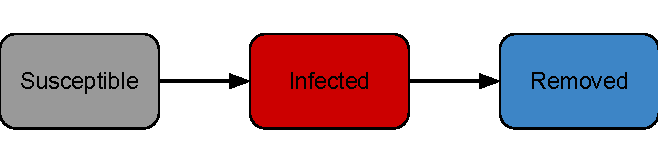
\includegraphics[height=3cm]{images/sir-idea}
	\end{figure}
	Usual assumptions:
	\begin{itemize}
		\item Population is \emph{homogeneous}
		\item Transmission is spatially iindependent
	\end{itemize}
\end{slide}